\documentclass[12pt]{beamer}

\usepackage[utf8]{inputenc}
\usepackage{graphicx}
\usepackage{wrapfig}
\usepackage{url}

\usetheme{Rochester}

\title{Unix - eine kurze Einführung}
\author{Kilian Gärtner, Rosario Raulin}
\date{Wintersemester 2012/13}

\begin{document}

\frame{\titlepage}

\begin{frame}
	\frametitle{Agenda}
	\tableofcontents
\end{frame}

\section{Geschichte}

\begin{frame}

	\frametitle{Geschichte (1)}

	\begin{columns}
		\begin{column}{0.7\textwidth}
			\begin{itemize}
				\item 1965 Mehrbenutzer-OS "Multics" vorgeschlagen
				\item ... scheiterte schnell an mangelnder Hardware
				\item Dennis Ritchie, K. Thompson, u. a. aber weiterhin interessiert
			\end{itemize}
		\end{column}


		\begin{column}{0.3\textwidth}
			\centerline{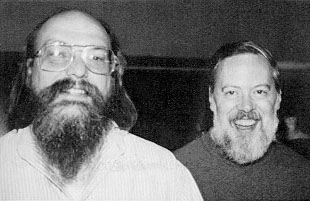
\includegraphics[scale=0.3]{src/img/thompson_richie}}
		\end{column}
	\end{columns}

\end{frame}

\begin{frame}
	
	\frametitle{Space Travel...}

	\begin{itemize}
		\item Thompson wollte Space Travel auf einer PDP-7 spielen
		\pause
		\item ... das ging aber nicht
		\pause
		\item also: "Wir hacken dann mal was"
		\pause
		\item Unix war geboren :)
	\end{itemize}

\end{frame}

\begin{frame}

	\frametitle{Geschichte (2)}

	\begin{columns}
		\begin{column}{0.3\textwidth}
			\centerline{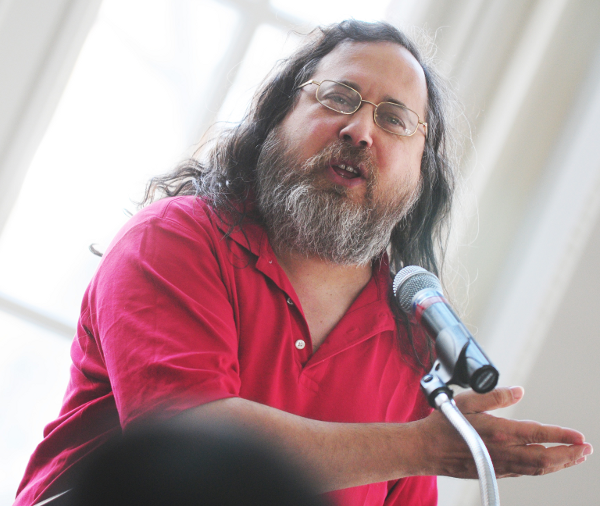
\includegraphics[scale=0.5]{src/img/rms}}
		\end{column}

		\begin{column}{0.7\textwidth}
			\begin{itemize}
				\item ab 1980: Unix-Verbreitung und -"Kriege"
				\item Richard Stallmann startet 83 das GNU-Projekt
				\item GNU = GNU's not Unix
				\item Freie-Software-Bewegung entsteht
			\end{itemize}
		\end{column}
	\end{columns}
\end{frame}

\begin{frame}

	\frametitle{Geschichte (3)}
	
	\begin{itemize}
		\item Anfang der 90er: GNU fast fertig, nur Kernel fehlt
		\item 1991/92: Linus Torvalds veröffentlicht "Linux"
		\item Resultat: keiner kennt GNU, alle sagen Linux
		\item Problem: Ideale des GNU-Projekts in Hintergrund gerückt
	\end{itemize}

	\begin{center}
		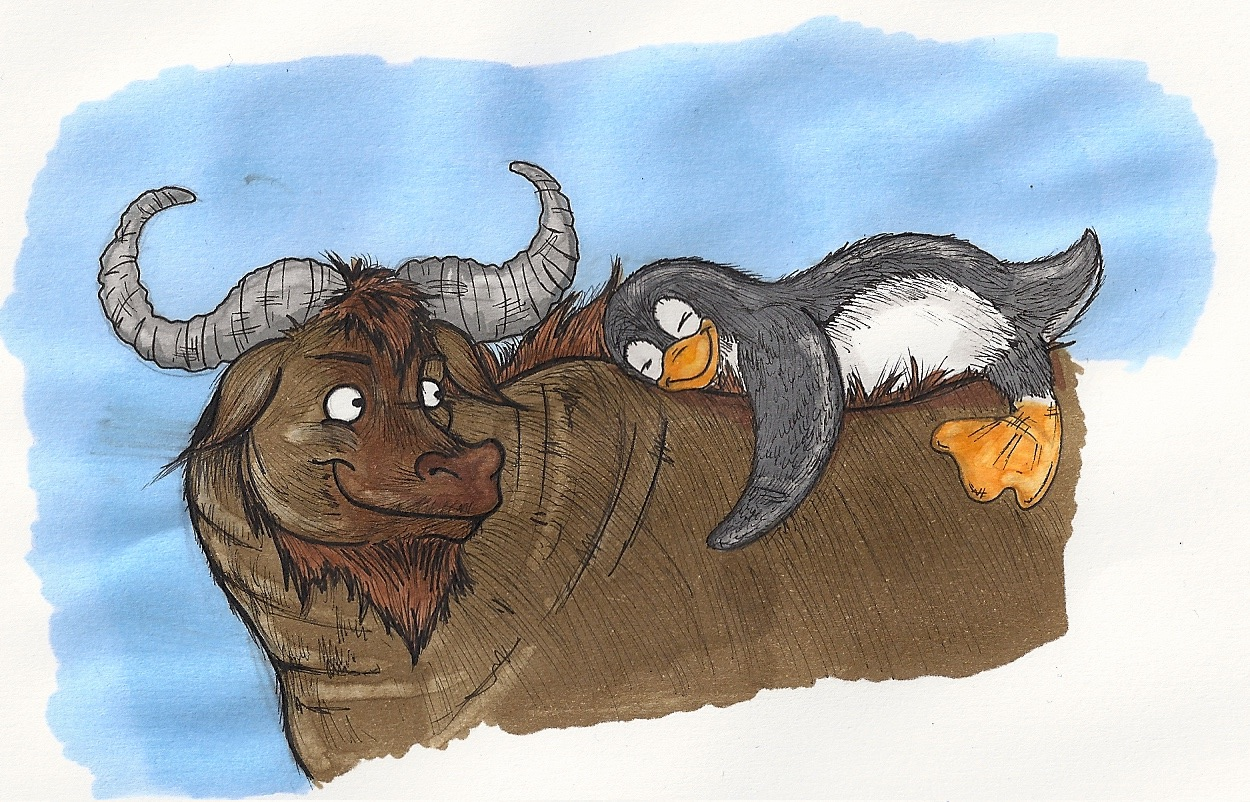
\includegraphics[scale=0.4]{src/img/gnulinux}
	\end{center}

\end{frame}

\section{Grundprinzipien}

\begin{frame}

	\frametitle{Die Unix-Philosophie}

	\begin{quote}
		Schreibe Computerprogramme so, dass sie nur eine Aufgabe erledigen
		und diese gut machen.

		\begin{flushright}
			\scriptsize Mcllroy (Erfinder der Unix-Pipes)
		\end{flushright}
	\end{quote}

	\pause

	und:
	\begin{itemize}
		\item\emph{Everything is a file}
		\item\emph{Premature optimization is the root of all evil}
		\pause
		\item\textbf{Die Shell}
	\end{itemize}
\end{frame}

\section{Die Shell}

\begin{frame}
	\frametitle{Warum überhaupt Texteingabe?}

	Weil...
	\begin{itemize}
		\pause
		\item weil es damals keine GUIs gab!
		\pause
		\item ihr 100 Bilder öffnen, verkleinern und schließen wollt
		\pause
		\item ... und das in einer Zeile geht! ;-)
	\end{itemize}
\end{frame}

\begin{frame}

	\frametitle{Grundbefehle der Shell}
	
	Einige Grundbefehle:
	\begin{itemize}
		\pause
		\item	ls - zeigt Dateien und Ordner
		\pause
		\item cd - wechselt das Verzeichnis
		\pause
		\item	cp - kopiert Dateien und Ordner (mit -r)
		\pause
		\item	mv - verschiebt Dateien und Ordner
		\pause
		\item rm - löscht Dateien und Ordner (mit -r)
		\pause
		\item mkdir - erstellt Ordner
		\pause
		\item cat - zeigt Dateiinhalte
		\pause
		\item exit - beendet die Shell
	\end{itemize}
\end{frame}

\begin{frame}

	\frametitle{Live-Demo (1)}

	1. Java-Programm in der Shell
	\begin{itemize}
		\item erstellen
		\item kompilieren
		\item ausführen
	\end{itemize}

\end{frame}

\begin{frame}
	\frametitle{Live-Demo (2)}

	2. Eclipse-Workspace von zu Hause per SCP holen:
	\begin{enumerate}
		\item scp -r \textdollar{}user@[1]:/home/\textdollar{}user/workspace \textdollar{}ziel
		\item	Passwort eintippen
		\item	Fertig!
	\end{enumerate}

	\scriptsize [1] \url{trex.cs.uni-magdeburg.de}
\end{frame}

\section{Fragen und Antworten}

\begin{frame}
	\frametitle{Fragen und Antworten}

	\begin{center}
		\large Gibt es Fragen?
	\end{center}
	\pause
	\centerline{\textbf{Vielen Dank für Eure Aufmerksamkeit!}}
\end{frame}

\end{document}

